%
% introduction.tex
%
% Copyright (C) 2022 by SpaceLab.
%
% OBDH 2.0 Module
%
% This work is licensed under the Creative Commons Attribution-ShareAlike 4.0
% International License. To view a copy of this license,
% visit http://creativecommons.org/licenses/by-sa/4.0/.
%

%
% \brief Introduction slides.
%
% \author Gabriel Mariano Marcelino <gabriel.mm8@gmail.com>
% \author Bruno Benedetti <brunobenedetti45@gmail.com>
%
% \version 0.1.0
%
% \date 2022/07/28
%

\begin{frame}{Overview}

    \begin{columns}[t]
        \begin{column}[t]{0.5\textwidth}
            \begin{itemize}
                \item On-Board Data Handling (OBDH) module for small satellites like CubeSats
                \vspace{0.3cm}
                \item Project name: ``\textit{OBDH 2.0}''
                \vspace{0.3cm}
                \item Custom made project
                \vspace{0.3cm}
                \item Fully open source
                \vspace{0.3cm}
                \item Based on FloripaSat-1 heritage
            \end{itemize}
        \end{column}
        \begin{column}[t]{0.5\textwidth}
            \begin{figure}[!ht]
                \begin{center}
                    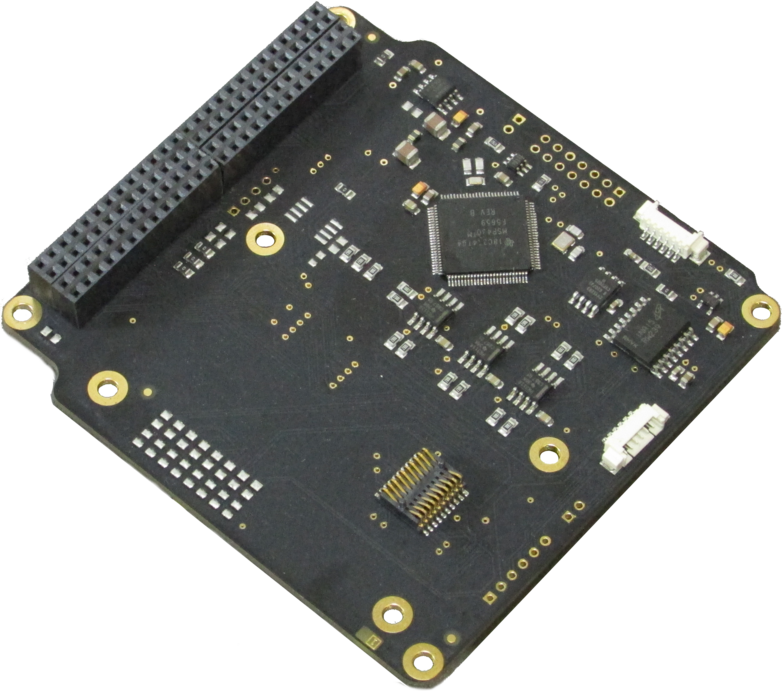
\includegraphics[width=5.5cm]{figures/obdh2-small.png}
                \end{center}
            \end{figure}
        \end{column}
    \end{columns}

\end{frame}

% #########################################################################
% #########################################################################

\begin{frame}{Product Tree}

    \begin{figure}[!ht]
        \begin{center}
            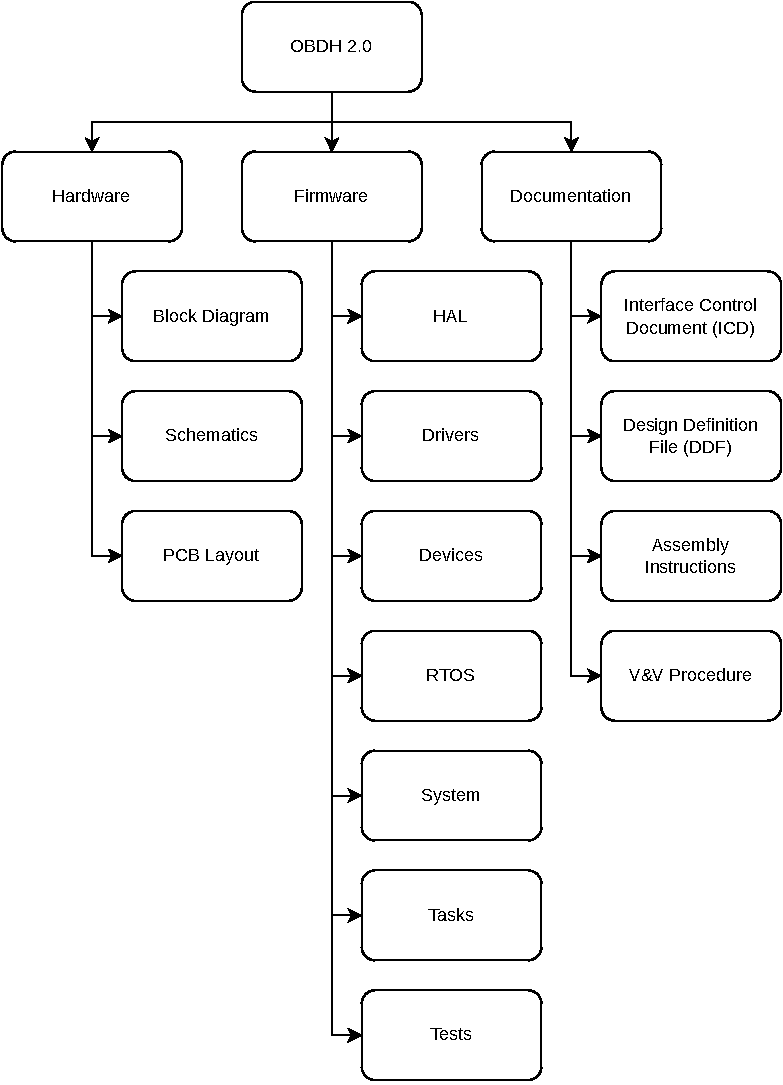
\includegraphics[width=5.5cm]{figures/product-tree}
        \end{center}
    \end{figure}

\end{frame}